\section{Análisis}

\subsection{Contexto}
\subsubsection{Descripción General}
Como todo proyecto el paso inicial es un análisis del objetivo a realizar, y este caso no es la excepción. La información utilizada para este análisis consistió en una explicación concisa de los requerimientos necesarios de la aplicación, principalmente mecánicas y características que debe contener la versión final, la cual concluyó que su desarrollo debe tener un énfasis en el funcionamiento básico de esta.\\
El resultado del análisis llevó a una descripción propia del proyecto, el resultado final es una aplicación que funcione como herramienta interactiva basada en una enseñanza de exploración y el contenido que esta acción entrega. La parte lúdica del aprendizaje se ve con la implementación de un sistema inspirado en juegos de mesa donde un numero plural de usuarios toman turnos para realizar acciones y avanzar en un mapa para llegar a una meta final. Cada turno se les entrega a los jugadores una imagen en 360 grados de un área o paisaje en particular y una cantidad de conceptos escogidos al azar (estas palabras son encontradas en una base de datos) con esto los usuarios tendrán que concebir una historia usando los datos mencionados. Al final todos tendrán que votar por otro usuario que consideren haber creado la mejor historia, el usuario ganador avanza un espacio y se sigue la misma idea cada turno hasta que uno llegue al final.
En cuanto a los problemas mencionados en el punto 1.1.2 se tomó la esquematización de estos y se analizaron con profundidad. La base de datos a utilizar debe centrarse en una cantidad reducida de usuarios (cuantos jugadores simultáneos se encuentran), también se llegó a la conclusión de que cada usuario cuenta con su propio dispositivo (un smartphone) por lo que se requerirá uso de internet para facilitar los datos a los usuarios. El análisis del proyecto y de la situación del equipo de desarrollo encuentra que el uso de Android studio (con el lenguaje de kotlin) y la implementación de firebase a este es la opción mas viable.\\
El diseño de la aplicación lleva a la conclusión de comenzar la estructura principal de este (encontrado en el caso de estudio entregado al equipo) dándole una mayór importancia la implementación las mecánicas claves recibidas, asegurándose de que estas funcionen sin problemas antes de ampliar o expandir el desarrollo del proyecto.
Lo que respecta a material audiovisual el equipo encarga en las ultimas fases de desarrollo un tiempo en particular para la búsqueda e implementación de sonidos o imágenes necesarias, y al igual que los otros casos, dándole mayor importancia a las direcciones entregadas al equipo, en este caso siendo el uso de imágenes en 360 grados en la aplicación.

\subsubsection{Descripción de Clientes y Usuarios:}
Luego de un análisis realizado en base a la información entregada del resultado esperado por la aplicación se a encontrado un perfil definido para tanto clientes como usuarios.
Los clientes son parte de el laboratorio mauletec y fueron concretados como un grupo centrado en una de las mecánicas principales presentadas. En específico, la vista de paisajes y lugares geográficos en 360 grados le interesa a un grupo enfocado en turismo como forma de enseñar los paisajes de una zona o región en particular. El otro enfoque encontrado en la aplicación que puede llamar la atención para un cliente es la mecánica de crear historias en base a palabras encontradas en una base de datos, tomando con mayor atención la parte literaria de juego centrada en la creatividad del usuario, pero siendo usada como forma de enseñanza.\\
Por otro lado, durante el desarrollo de la aplicación los usuarios tomaron un enfoque más genérico que el de los clientes, se encontró que en cualquier caso estos tenían requerimientos  simples ya que lo más importante es facilitarles el uso de esta. El usuario objetivo se identificó como un individuo o individua con un conocimiento basico de tecnologia, tomando en cuenta de que la plataforma utilizada es de smartphones. Ademas se contar con un dispositivo que cuente con un sistema operativo que permita instalar y usar la aplicación, se requiere que el usuario entienda el concepto de identificarse de forma virtual con su correo electronico ademas de entender las reglas básicas del juego. Además, este debe tener un conocimiento literario de enseñanza básica como mínimo, tomando en cuenta de que la interacción principal de parte del usuario es crear y contar una historia en base a un grupo de palabras entregadas.
\subsection{Especificación de Requerimientos}
\subsubsection{Funciones del Sistema}
Funciones evidentes:
\\	-Registrar nuevo usuario.
\\	-Realizar autentificacion con correo.
\\	-Realizar autentificacion con contraseña.
\\	-Realizar autentificacion con Gmail.
\\	-Mostrar imagenes en 360°.
\\	-Sistema de turnos.
\\	-Generar lista de palabras.
\\	-Multijugador global.


Funciones ocultas:
\\	-Cargar imagenes en 360°.
\\	-Crear base de datos para palabras.
\\	-Crear base de datos para puntajes.


Funciones Supérfluas:
\\	-Generar una tabla de puntajes.
\subsubsection{Atributos del Sistema}
-Intuitiva: Debe ser de facil entendimiento para el usuario final, es decir, el ususario debe saber que hacer o como empezar a jugar sin mucha complejidad.


-Optimizado: La aplicación debe usar recursos del celular solo de ser sumamente necesario.


-Baja frecuencia de fallos: El Programa no debe presentar mas de cuatro fallos al mes.


-Facilidad de configuración: Debe ser sencillo para el usuario customizar a su gusto la aplicacion.


-Facilidad de mantenimiento: A los programadores y gente encargada de mantener la aplicacion dfuncionando se les debe hacer sencillo ingresar al codigo, entenderlo y aplicar las reparaciones
\subsubsection{Atributos por Función}
\begin{table}[H]
    \begin{center}
        \begin{tabular}{| l | m{6cm} | m{6cm} |}        
        	\hline 
        	Ref\# & Función & Atributo\\
        	\hline
        	R1.1 & Registrar nuevo usuario & Facilidad de configuración\\
        	\hline
        	R1.2 & Realizar autentificacion con correo, contraseña o gmail & Facilidad de configuración\\
        	\hline
        	R1.3 & Mostrar imagenes en 360° & Intuitiva\\
        	\hline
        	R1.4 & Sistema de turnos & Intuitiva\\
        	\hline
        	R1.5 & Generar lista de palabras & Intuitiva\\
        	\hline
        	R1.6 & Multijugador global & Facilidad de configuracion\\
        	\hline
        	R1.7 & Cargar imagenes 360° & Facilidad de configuración\\
        	\hline
        	R1.8 & Crear base de datos para palabras y puntaje & Facilidad de mantenimiento\\
        	\hline
        \end{tabular}
    \caption{Funciones agrupadas}
    \end{center}
\end{table}
\newpage
\subsection{Actores}
Jugador : La aplicación está hecha para que sea utilizada por usuarios, su último fin es entretener a un público y es quien debiera ser su actor final y principal.

2. Autores : Son quienes se encargan de dar mantencion y programar la aplicacion para su correcto funcionamiento.

3. FireBase : Permite el contacto entre la aplicación y múltiples herramientas como lo son la base de datos, el guardado de respaldo, etc. Además hace nexo entre la aplicación y los siguientes actores:

a. -Base de Datos : La aplicación debe mantener contacto con la base de datos de forma directa, para poder acceder a las palabras, imágenes, usuarios, etc.

b. -Gmail : Herramienta principal para identificar al usuario por medio de correo electrónico.
\subsection{Casos de Uso}
\begin{table}[H]
    \begin{center}
        \begin{tabular}{| l | m{12cm} |}        
        	\hline 
        	Identificador & 1\\
        	\hline
        	Caso de Uso & Jugar una partida de Conquista Turística
360°\\
        	\hline
        	Actores & Jugador\\
        	\hline
        	Propósito & Jugar un turno\\
        	\hline
        	Tipo & Primario y escencial\\
        	\hline
        	Descripción & El programa le muestra al jugador 4 palabras por pantalla, el jugador las ve y las usa para crear una historia. Los demás jugadores votan por la creatividad de la historia en la applicacion y deciden que el jugador puede avanzar, el programa recibe el feedback de los jugadores por pantalla y mueve al jugador a la siguiente posición.\\
        	\hline
        	Referencias Cruzadas & R1.4 ,R1.5 ,R1.6\\
        	\hline
        \end{tabular}
    \caption{Primer caso de uso}
    \end{center}
\end{table}

\begin{table}[H]
    \begin{center}
        \begin{tabular}{| l | m{12cm} |}        
        	\hline 
        	Identificador & 2\\
        	\hline
        	Caso de Uso & Iniciar sesión\\
        	\hline
        	Actores & Jugador y FireBase\\
        	\hline
        	Propósito & Entrar en su cuenta personal\\
        	\hline
        	Tipo & Primario y Real\\
        	\hline
        	Descripción & El jugador abre la aplicación he ingresa sus datos, la aplicación los recibe y los compara en la base de datos a traves del FireBase, si la informacion es correcta el jugador ingresa a la pantalla principal \\
        	\hline
        	Referencias Cruzadas & R1.1 ,R1.2\\
        	\hline
        \end{tabular}
    \caption{Segundo caso de uso}
    \end{center}
\end{table}

\begin{table}[H]
    \begin{center}
        \begin{tabular}{| l | m{12cm} |}        
        	\hline 
        	Identificador & 3\\
        	\hline
        	Caso de Uso & Generar lista de palabras\\
        	\hline
        	Actores & Jugador y FireBase\\
        	\hline
        	Propósito & Entregar palabras para que el jugador pueda intervenir\\
        	\hline
        	Tipo & Primario y escencial\\
        	\hline
        	Descripción & El jugador toca la imagen 360° y la aplicacion accede a la base de datos a traves del FireBase, busca 4 palabras aleatorias y se las muestra al jugador por pantalla\\
        	\hline
        	Referencias Cruzadas & R1.3 ,R1.5\\
        	\hline
        \end{tabular}
    \caption{Tercer caso de uso}
    \end{center}
\end{table}

\begin{table}[H]
    \begin{center}
        \begin{tabular}{| l | m{12cm} |}        
        	\hline 
        	Identificador & 4\\
        	\hline
        	Caso de Uso & Mostrar imagen 360°\\
        	\hline
        	Actores & Jugador\\
        	\hline
        	Propósito & Retroalimentar al jugador \\
        	\hline
        	Tipo & Primario y escencial\\
        	\hline
        	Descripción & Cuando el jugador conquista una posición, avanza a la siguiente y el programa le presenta a traves de una imagen 360° su nuevo objetivo\\
        	\hline
        	Referencias Cruzadas & R1.3\\
        	\hline
        \end{tabular}
    \caption{Cuarto caso de uso}
    \end{center}
\end{table}

\begin{table}[H]
    \begin{center}
        \begin{tabular}{| l | m{12cm} |}        
        	\hline 
        	Identificador & 5\\
        	\hline
        	Caso de Uso & Mostrar tabla de puntajes\\
        	\hline
        	Actores & Jugador y FireBase\\
        	\hline
        	Propósito & Retroalimentar al jugador\\
        	\hline
        	Tipo & Secundario y real\\
        	\hline
        	Descripción & El jugador accede a la tabla de puntajes y el programa a su ves ingresa a la base de datos a traves del FireBase donde estan almacenados todos los puntajes y se los presenta al jugador de manera ordenada\\
        	\hline
        	Referencias Cruzadas & R1.8\\
        	\hline
        \end{tabular}
    \caption{Quinto caso de uso}
    \end{center}
\end{table}

\begin{table}[H]
    \begin{center}
        \begin{tabular}{| l | m{12cm} |}        
        	\hline 
        	Identificador & 6\\
        	\hline
        	Caso de Uso & Cargar imagen 360°\\
        	\hline
        	Actores & Autores\\
        	\hline
        	Propósito & Retroalimentar al jugador\\
        	\hline
        	Tipo & Principal y escencial\\
        	\hline
        	Descripción & Los autores del programa Editan y ajustan la imagen para que quede de acorde a las especificaciones del sistema y luego la cargan a la aplicación\\
        	\hline
        	Referencias Cruzadas & R1.7\\
        	\hline
        \end{tabular}
    \caption{Sexto caso de uso}
    \end{center}
\end{table}
\subsubsection{Caso de Uso Esencial}

\subsubsection{Diagrama de Caso de Uso}
\subsubsection{Contrato}
\subsubsection{Modelo Conceptual}
\subsubsection{Diagrama de Secuencia o Colaboración}
\begin{figure}[htbp]
\centering
   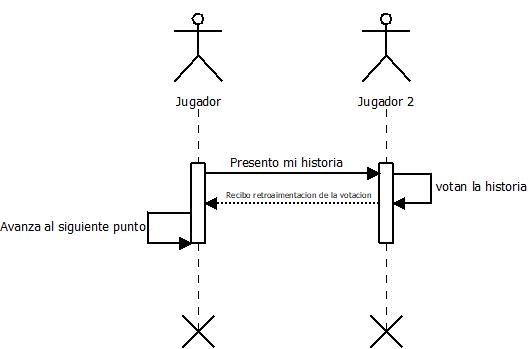
\includegraphics[scale=0.9]{imgs/DS_1.jpeg}
   \begin{center}
   Diagrama de secuencia: Primer caso de uso
   \end{center}
\end{figure}

\begin{figure}[htbp]
\centering
   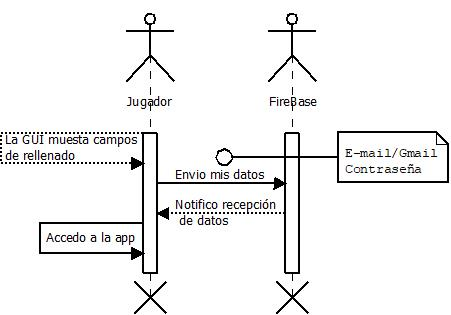
\includegraphics[scale=0.9]{imgs/DS_2.jpeg}
   \begin{center}
   Diagrama de secuencia: Segundo caso de uso
   \end{center}
\end{figure}

\begin{figure}[htbp]
\centering
   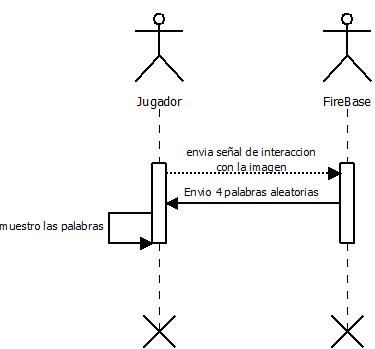
\includegraphics[scale=0.9]{imgs/DS_3.jpeg}
   \begin{center}
   Diagrama de secuencia: Tercer caso de uso
   \end{center}
\end{figure}

\begin{figure}[htbp]
\centering
   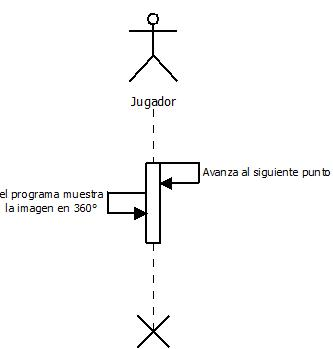
\includegraphics[scale=0.9]{imgs/DS_4.jpeg}
   \begin{center}
   Diagrama de secuencia: Cuarto caso de uso
   \end{center}
\end{figure}

\begin{figure}[htbp]
\centering
   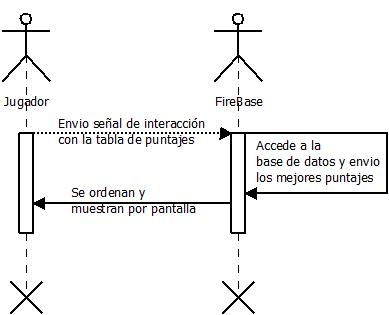
\includegraphics[scale=0.9]{imgs/DS_5.jpeg}
   \begin{center}
   Diagrama de secuencia: Quinto caso de uso
   \end{center}
\end{figure}

\begin{figure}[htbp]
\centering
   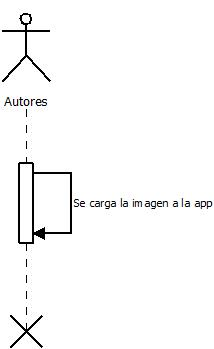
\includegraphics[scale=0.9]{imgs/DS_6.jpeg}
   \begin{center}
   Diagrama de secuencia: Sexto caso de uso
   \end{center}
\end{figure}
\subsubsection{Priorización}

\subsection{Modelo de Dominio}
\subsubsection{Entidades Reconocidas}
\subsubsection{Modelo de Dominio}
\subsubsection{Matriz de Rastreabilidad}